% Chapter 3

\chapter{Results} % Main chapter title
\label{Chapter3} % For referencing the chapter elsewhere, use \ref{Chapter3} 
\addtocontents{toc}{\setcounter{tocdepth}{1}}
\section{Assessment of inducible GLUT1 expression}
Previous results from the work of our laboratory showed that the GLUT1\textsuperscript{P485L} mutation leads to specific interaction with clathrins and the internalization of the protein. In order to further investigate the role and functional effects of the mutation, we generated two Flp-In T-Rex HEK293 cell lines containing inducible BirA-FLAG epitope-tagged full length wild-type or mutant GLUT1 (Figure~\ref{fig:vectors}). The cells constitutively express Tet repressor (TetR) which binds to the TetO\textsubscript{2} sequence in the promoter of transgenic GLUT1~\cite{Hillen}. Upon addition, tetracycline binds to the TetR, causing the release of TetR from TetO\textsubscript{2} and induction of transgene transcription~\cite{Hillen}. In this thesis doxycycline was used as a relatively stable tetracycline derivative to induce the expression of the BirA-FLAG tagged GLUT1 variants~\cite{Xu}.

To determine the optimal conditions for inducible expression, GLUT1 wild-type and mutant cells were grown in different concentrations of doxycycline for 24 hr and the expression of the GLUT1 protein was analyzed by Western blotting with an anti-FLAG antibody. No GLUT1 expression was detected in the absence of doxycycline (Figure~\ref{fig:wb} A). Compared with 0.1 \textmu g/mL doxycycline, induction with 1 \textmu g/mL doxycycline resulted in higher GLUT1 levels in wild-type cells, whereas in mutant cells the GLUT1 expression was not significantly altered (Figure~\ref{fig:wb}, A and C). The results showed that the lower dose of doxycycline was sufficient for induction of the system. 

Additionally, GLUT1 protein expression was quantified after 24 hr and 48 hr of doxycycline induction. Further increase in the induction time did not result in increased GLUT1 levels in wild-type cells, but actually decreased the expression in mutant cells compared to the 24 hr time point (Figure~\ref{fig:wb}, B and D). Therefore the induction with 0.1 \textmu g/mL doxycycline for 24 hr was selected in the following experiments to reduce toxic side effects of the drug~\cite{Zeltser}.

\begin{figure}[h]
\centering
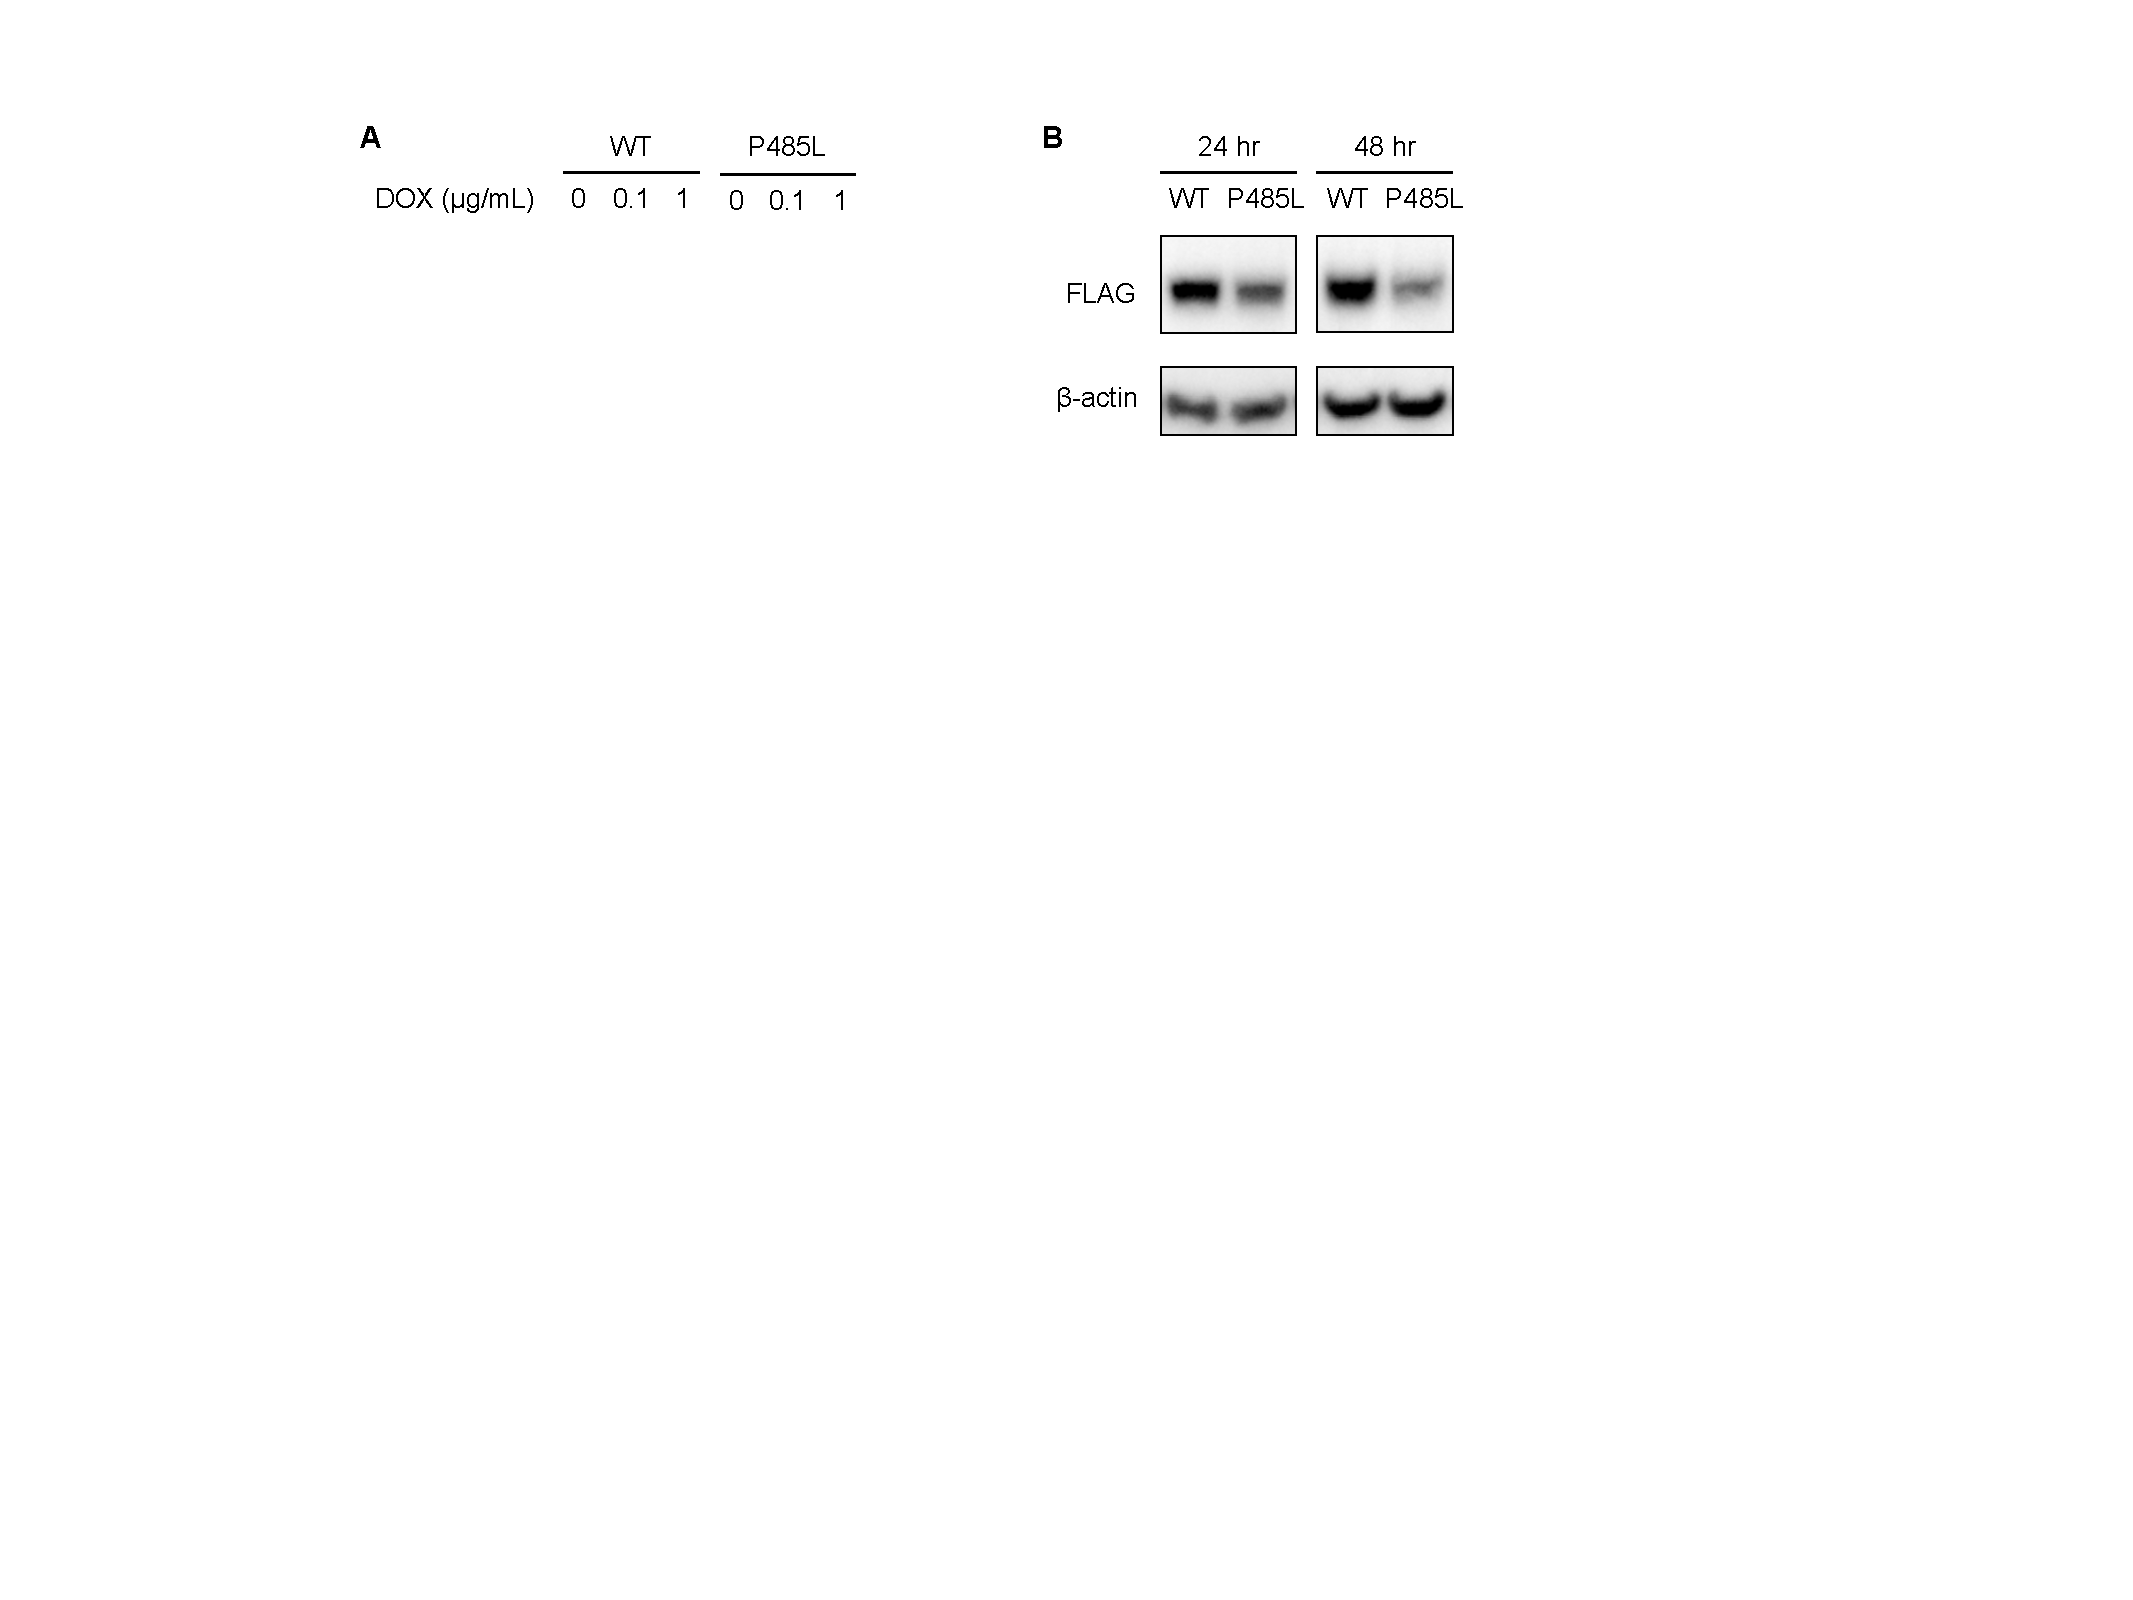
\includegraphics[scale=0.7]{Figures/WB}
\caption{The doxycycline-inducible expression of GLUT1 variants.}
%\smallskip
\vspace*{-3mm}
\small \justify
Different conditions were investigated to induce the expression of BirA-FLAG tagged GLUT1 with doxycycline. GLUT1 wild-type (WT) and mutant (P485L) cells were treated with varying concentrations of doxycycline (0, 0.1 or 1 \textmu g/mL) for 24 hr and analyzed with Western blotting (A). The inducible expression of GLUT1 was also compared between 24 hr and 48 hr induction with 0.1 \textmu g/mL doxycycline (B). Quantification of GLUT1 levels was achieved by normalizing to \textbeta -actin (C, D).
\label{fig:wb}
\end{figure}
Furthermore, the doxycycline-inducible expression of GLUT1 was confirmed by immunofluorescence confocal microscopy. A different anti-FLAG antibody was used to analyze transgene expression with or without doxycycline treatment in both cell lines. Interestingly, although leakiness in expression was not detected in Western blotting, a small subpopulation of uninduced wild-type and mutant cells showed transgene expression in immunofluorescence microscopy (Figure~\ref{fig:if}, A and B). In addition, a low basal expression of FLAG-tagged GLUT1 was visible under stronger laser excitation in uninduced wild-type cells,
% Supplementary fig???, 
suggesting the existence of leaky expression from the Tet promoter in the absence of doxycycline~\cite{Pham,Senkel}. 
In consistence with Western blotting results, strong and roughly uniform expression in response to doxycycline was observed in wild-type and mutant cells (Figure~\ref{fig:if}, C and D). 
\begin{figure}[h]
\centering
\includegraphics[scale=0.7]{Figures/if}
\caption{The inducible expression of GLUT1 variants assessed by immunofluorescence microscopy.}
\vspace*{-3mm}
\small \justify
GLUT1 wild-type (WT) and mutant (P485L) cells were cultured on coverslips for 24 hr either in the absence (A, B) or presence (C, D) of 0.1 {}\textmu g/mL doxycycline. Immunostaining of BirA-FLAG tagged GLUT1 was performed with monoclonal mouse anti-FLAG and Alexa 488-conjugated anti-mouse antibodies (green). Cell nuclei were identified by DAPI staining (blue). Scale = 10 \textmu m.
\label{fig:if}
\end{figure}
%As expected, ARF localized to nucleolar regions (the compact circular regions of higher intensity as pointed by the arrow in panel A) while HA-RBP1 demonstrated strong nuclear localization with nucleolar exclusion, as shown by the dark nucleolar regions in panel B. Panel C confirms that RBP2 is localized exclusively to the nucleus. Panel D illustrates that the rabbit polyclonal ?-RBP2 antibody cannot be used in immunofluorescence because of the high amount of non-specific background signal it produces. Trials were done at various dilutions but all were negative and produced the same non-specific noise (data not shown). 

\section{Effect of blocking proteolysis on GLUT1 levels}
Despite the approximately uniform expression within both cell lines, a lower level of GLUT1 expression was observed in mutant cells than in wild-type cells (FIgure~\ref{fig:wb}). We thus speculated that the mutant protein might undergo degradation through proteolytic pathways. A rescue experiment was designed to determine the effect of proteolysis on GLUT1 levels by using proteolytic inhibitors Bafilomycin A1 or MG132 to block lysosomal degradation or proteosomal degradation, respectively~\cite{Tanida,Lee.2}. The GLUT1 levels in cells with or without inhibitor treatment were quantified by Western blotting analyses.
%(Figure~\ref{fig:wb2}). 

Bafilomycin A1 inhibits the vacuolar type H\textsuperscript{+}-ATPase complex necessary for lysosomal acidification, thus blocks protein degradation in lysosomes~\cite{Yamamoto,Klionsky}. The inhibitory effect of Bafilomycin A1 was confirmed by the accumulation of LC3-phosphatidylethanolamine conjugate (LC3-II) upon inhibitor treatment (Figure~\ref{fig:wb2} A). Surprisingly, the inhibition decreased wild-type GLUT1 levels by approximately 10\% in comparison to the untreated control group, whereas in mutant cells the inhibition increased GLUT1 levels by around 30\% (Figure~\ref{fig:wb2} B). These results suggest that lysosomal degradation might be partially responsible for the differential GLUT1 protein levels in the two cell lines, but independent sets of experiments and quantifications need to be repeated.

\begin{figure}[h]
\centering
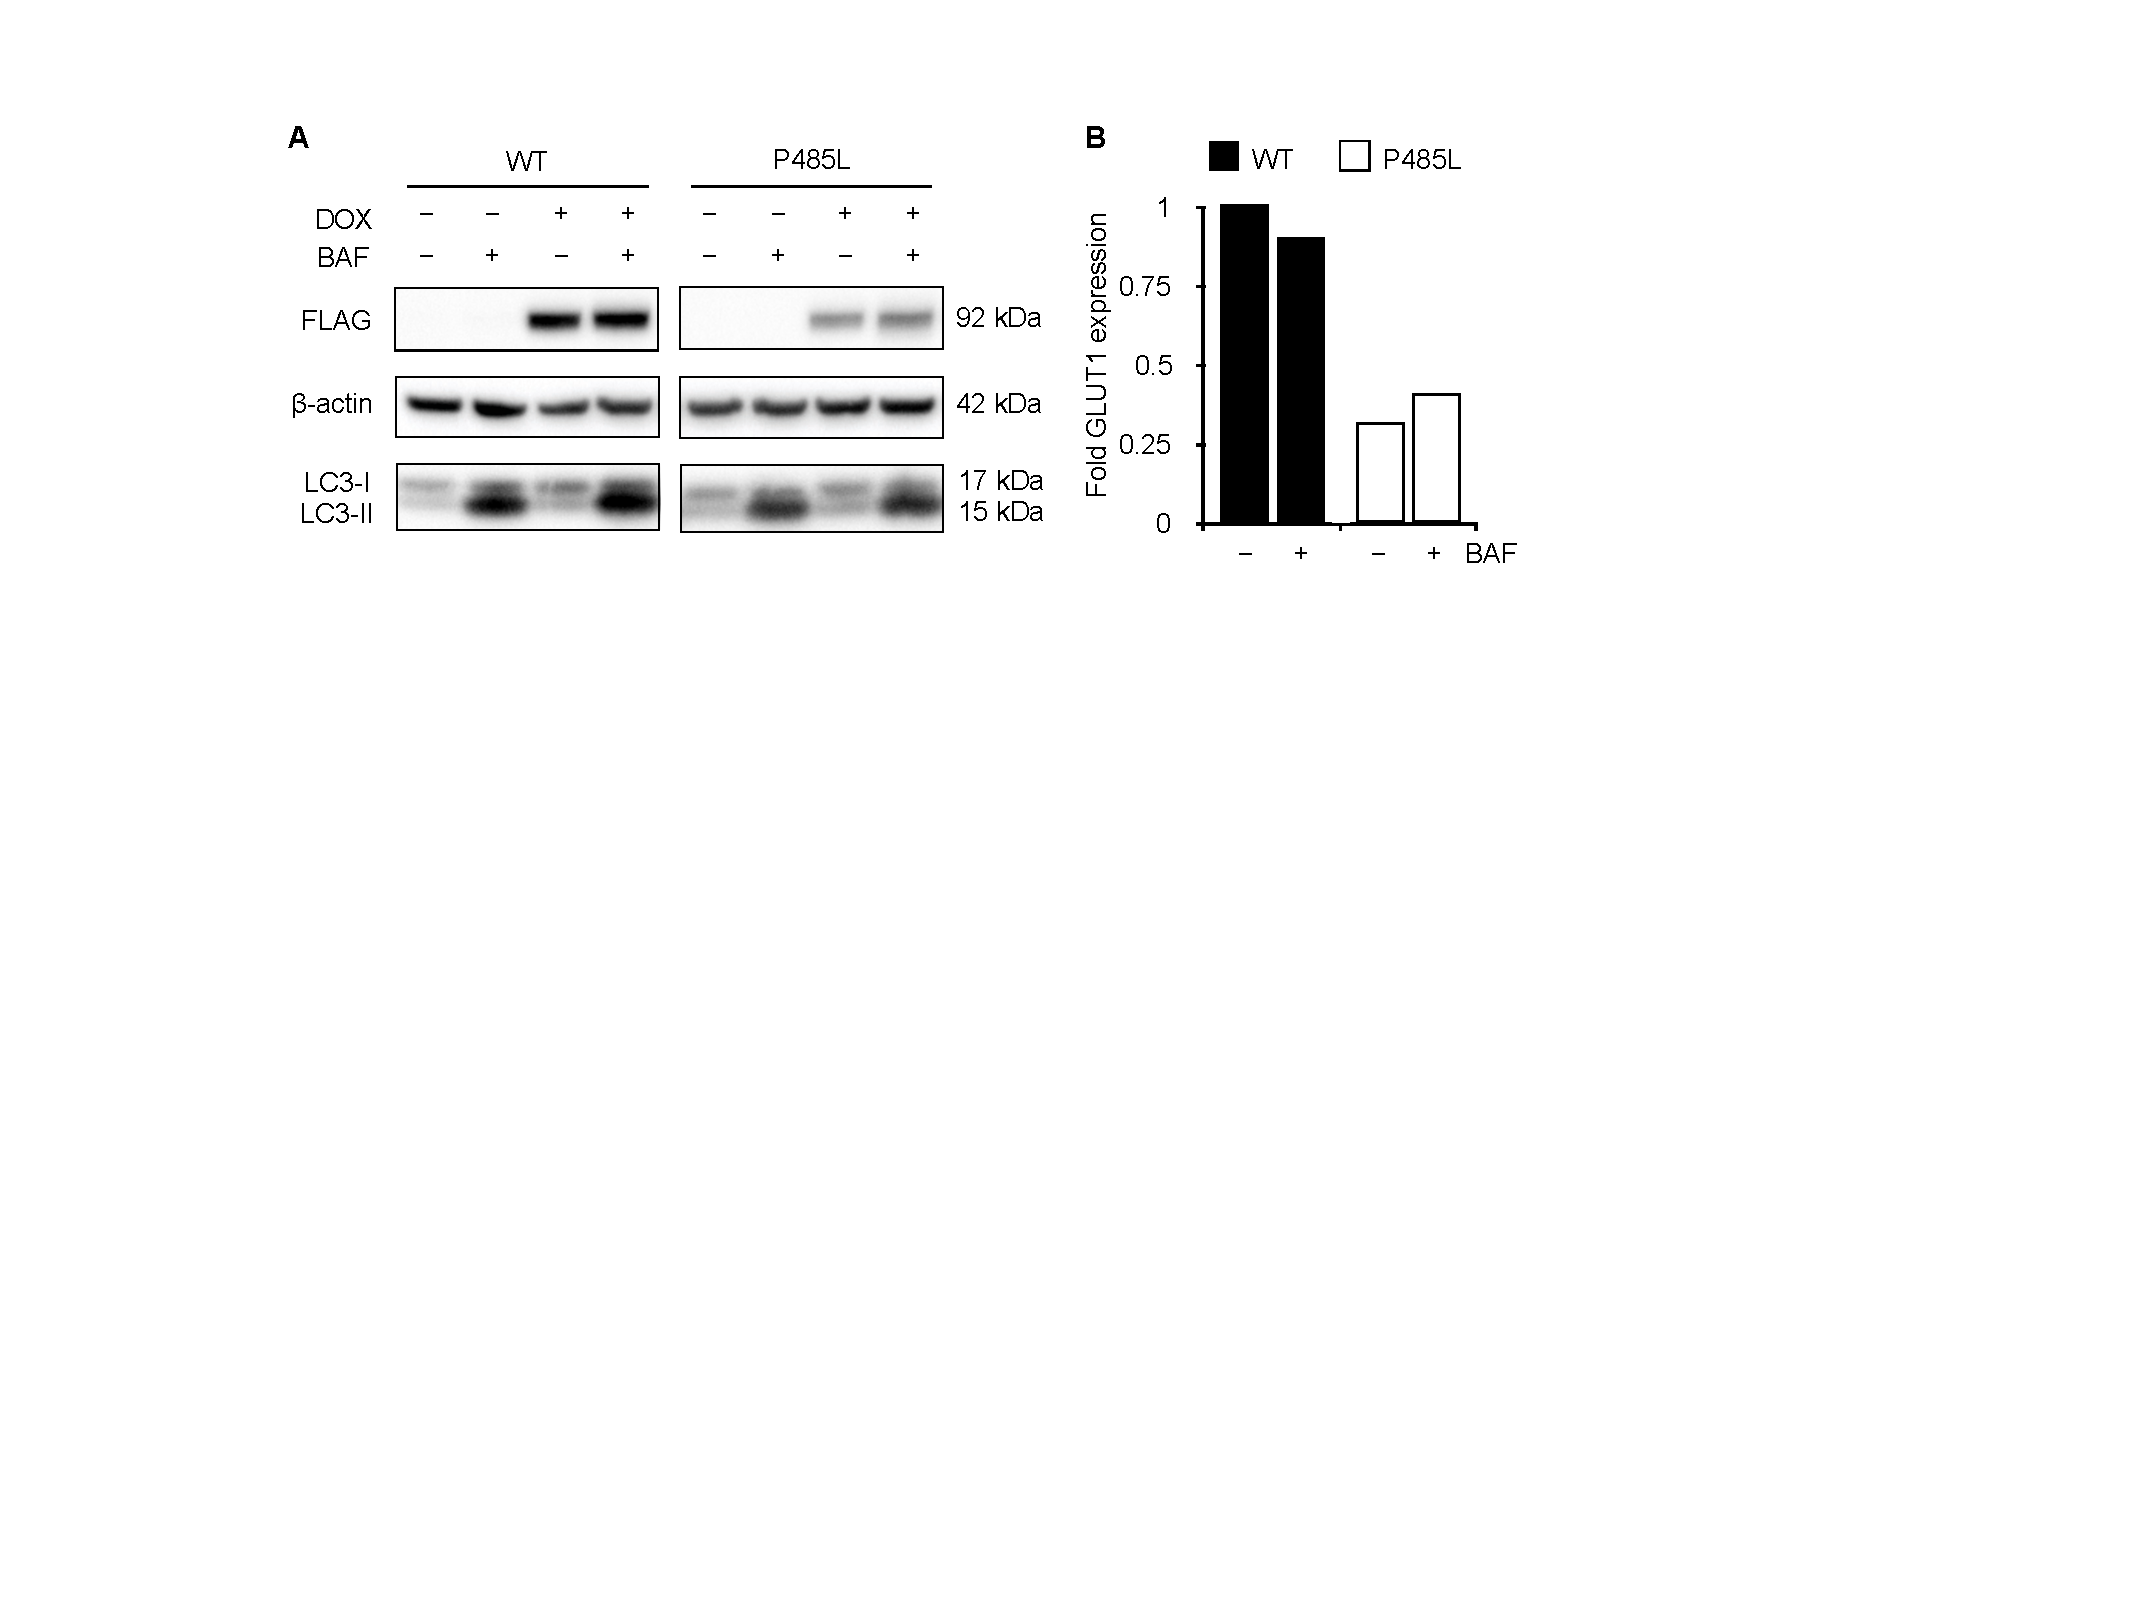
\includegraphics[scale=0.7]{Figures/wb2}
\caption{The effect of blocking lysosomal degradation on GLUT1 levels.}
\vspace*{-3mm}
\small \justify
GLUT1 wild-type (WT) and mutant (P485L) cells were incubated in 0.1 \textmu g/mL doxycycline for 18 hr before Bafilomycin A1 (BAF, final concentration: 250 nM) or carrier control (DMSO) was added. After 6 hr of drug treatment, the cells were lysed and the GLUT1 levels were analyzed in Western blotting (A). Quantification of GLUT1 levels in induced cells was achieved by normalizing to \textbeta -actin (B).
\label{fig:wb2}
\end{figure}
To demonstrate that the proteosomal inhibitor MG132 did decrease proteosomal degradation, cells were transfected with HA epitope-tagged UL21a after doxycycline induction. UL21a has been reported to encode the viral protein pUL21a, a short-lived cytoplasmic protein targeted for proteosome-dependent degradation and can be drastically stabilized in the presence of MG132~\cite{Fehr}. The cells were treated with MG132 or DMSO control after UL21a transfection, and analyzed for the accumulation of HA-tagged pUL21a and FLAG-tagged GLUT1 levels by Western blotting. The accumulation of pUL21a was observed after MG132 treatment, but no significant effect of proteosomal inhibition was shown on wild-type and mutant GLUT1 levels (Figure~\ref{fig:wb3}).

\begin{figure}[h]
\centering
\includegraphics[scale=0.7]{Figures/wb3}
\caption{The effect of blocking proteosomal degradation on GLUT1 levels.}
\vspace*{-3mm}
\small \justify
GLUT1 wild-type (WT) and mutant (P485L) cells were incubated in 0.1 \textmu g/mL doxycycline for 1 hr before being transfected with HA-UL21a. At 17 hr after transfection, MG132 (final concentration: 20 mM) or DMSO control. Cells lysates were collected 6 hr later and analyzed by immunoblotting with an anti-FLAG antibody to determine GLUT1 levels and an anti-HA antibody for pUL21a levels (A). The GLUT1 level in doxycycline induced cells were quantified by normalizing to \textbeta -actin (B).
\label{fig:wb3}
\end{figure}
%we examined LC3-II or p62 levels in serum-starved cellseither in the absence, or presence of bafilomycin A1, an agent thatinhibits lysosomal acidification and/or inhibits autophagosome-lysosome fusion; this treatment leads to reduced degradation andhence, accumulation of autophagy substrates A Role for Presenilins in Autophagy Revisited: Normal Acidification of Lysosomes in Cells Lacking PSEN1 and PSEN2 (PDF Download Available). Available from: https://www.researchgate.net/publication/227858130_A_Role_for_Presenilins_in_Autophagy_Revisited_Normal_Acidification_of_Lysosomes_in_Cells_Lacking_PSEN1_and_PSEN2 [accessed Jul 13, 2017].
%LC3-II levels were elevated in cultured WT-ES cells(Fig. 1A, compare lanes 1, 2)
\section{Cellular localization of GLUT1 variants}
The plasma membrane localization of wild-type GLUT1 has been well demonstrated in sequence and structural studies~\cite{Mueckler.2,Hresko,Hruz}.
To compare the localization of wild-type and mutant GLUT1, we examined the localization in the two stable cell lines by immunofluorescent microscopy. Expression of the FLAG-tagged wild-type GLUT1 was clearly detected on the cell surface (Figure~\ref{fig:glut1} B). Conversely, the FLAG-tagged mutant GLUT1 was mostly expressed in intracellular regions (Figure~\ref{fig:glut1} D). Additionally, this differential localization was confirmed by using an anti-GLUT1 antibody (Figure~\ref{fig:glut1} A and C).

\begin{figure}[h]
\centering
\includegraphics[scale=0.7]{Figures/glut1}
\caption{The differential cellular localization of GLUT1 variants.}
\vspace*{-3mm}
\small \justify
Localization of GLUT1 wild-type (WT) and mutant (P485L) was analyzed in HEK293 cells induced with 0.1 \textmu g/mL doxycycline for 24 hr. Immunostaining of the FLAG-tagged GLUT1 variants was performed with rabbit anti-GLUT1 and Alexa 488-conjugated anti-rabbit antibodies (green, A and D), as well as mouse anti-FLAG and Alexa 568-conjugated anti-mouse antibodies (red, B and E). The overlay images with DAPI-stained nuclei were also shown (C and F). Scale = 10 \textmu m.
\label{fig:glut1}
\end{figure}
\section{Proximity labeling of GLUT1 variants}

\section{Co-localization study of GLUT1 variants}
\begin{figure}[h]
\centering
\includegraphics[scale=0.7]{Figures/tf}
\caption{The mutant GLUT1 co-localizes with endocytosed transferrin.}
\vspace*{-3mm}
\small \justify
But not the wild-type GLUT1. Scale = 10 \textmu m.
\label{fig:tf}
\end{figure}

%----------------------------------------------------------------------------------------
% Define some commands to keep the formatting separated from the content 
